\PassOptionsToPackage{table}{xcolor}
\documentclass{article}
\usepackage[colorlinks]{hyperref}
\usepackage[margin=1.25in]{geometry}
\usepackage{amsmath,amssymb,amsthm,booktabs,tikz}
\usepackage[final]{microtype}
\usepackage{libertine}
\usepackage[varqu]{zi4}
\usepackage[libertine]{newtxmath}
\usepackage[T1]{fontenc}
\usepackage[utf8]{inputenc}
\usepackage{tabto}
\usepackage[normalem]{ulem}

\usetikzlibrary{shapes.multipart}

% Seven colors safe for use color blindness.
% Colors taken from doi:10.1038/nmeth.1618.
\definecolor{cbOrange}{RGB}{230,159,0}
\definecolor{cbSkyBlue}{RGB}{86,180,233}
\definecolor{cbBluishGreen}{RGB}{0,158,115}
\definecolor{cbBlue}{RGB}{0,114,178}
\definecolor{cbVermillion}{RGB}{213,94,0}
\definecolor{cbReddischPurple}{RGB}{204,121,167}
\definecolor{cbYellow}{RGB}{240,228,66}

\theoremstyle{definition}
\newtheorem{problem}{Problem}
\newenvironment{questions}{\begin{enumerate}
\renewcommand{\theenumi}{P\arabic{problem}.\arabic{enumi}}}{\end{enumerate}}
\newcommand{\HL}[1]{\textcolor{cbReddischPurple}{#1}}

\newcommand{\abs}[1]{\lvert #1 \rvert}
\newcommand{\OOG}[1]{\mathord{\sim}#1}
\DeclareMathOperator{\bdiv}{div}

\newcommand{\BigO}[1]{\mathcal{O}\left(#1\right)}
\newcommand{\BigOmega}[1]{\Omega\left(#1\right)}
\newcommand{\BigTheta}[1]{\Theta\left(#1\right)}


\newcommand{\True}{\texttt{true}}
\newcommand{\False}{\texttt{false}}

%% Tikz
\usepackage{tikz}
\usetikzlibrary{arrows.meta,calc,decorations.pathreplacing,shapes.geometric,shapes.multipart,overlay-beamer-styles}
\tikzset{
    >=Stealth,
    dot/.style={circle,scale=0.35,draw=black,fill=black},
    stacked/.style={above,rectangle split,draw,rectangle split parts=#1,font=\strut,rectangle split part fill={none,black!10}},
    centered/.append style={align=center}
}


% Algorithm
\usepackage{algorithmic}
\newcommand{\GETS}{:=}
\newcommand{\VAR}[1]{\textit{#1\/}}
\newcommand{\AName}[1]{\textsc{#1}}
\renewcommand{\algorithmicrequire}{\textbf{Input:}}
\renewcommand{\algorithmicensure}{\textbf{Result:}}
\newcommand{\CMT}[1]{\text{``#1''}}
\renewcommand{\algorithmiccomment}[1]{\CMT{#1}}
\newcommand{\INV}[1]{\emph{inv: } #1}
\newcommand{\VF}[1]{\emph{bf: } #1}
\makeatletter
\newlength{\Algo@MyTabLength}
\newcommand{\AlgoTabTo}[1]{%
    \setlength{\Algo@MyTabLength}{#1}%
    \addtolength{\Algo@MyTabLength}{-\ALC@tlm}%
    \tabto{\Algo@MyTabLength}%
}
\newenvironment{myonlyalgo}[1][0]{
    \vskip 5pt
    \hrule
    \smallskip
    \begin{algorithmic}[1]
    \setcounter{ALC@line}{#1}
}{
    \end{algorithmic}
    \hrule
    \vskip 5pt
}
\newenvironment{myalgo}[2][0]{
    \vskip 5pt
    \hrule
    \smallskip
    \noindent{\textbf{Algorithm} #2\textbf{:}}
    \begin{algorithmic}[1]
    \setcounter{ALC@line}{#1}
}{
    \end{algorithmic}
    \hrule
    \vskip 5pt
}







%% Metadata
\newcommand{\Assignment}[1]{
    \title{\vskip-2em%The standard article.cls package puts 2em whitespace on top of the title, undo this.
           Assignment #1\\{\Large SFWRENG 2CO3: Data Structures and Algorithms--Winter 2023}}}
\newcommand{\Deadline}[1]{
    \author{Deadline: #1}
}
\date{{\normalsize
    Department of Computing and Software\\
    McMaster University
}}

\newcommand{\Warning}[1]{\textbf{\textcolor{red!80!black}{#1}}}
\renewcommand{\labelitemi}{$\blacktriangleright$}

\newcommand{\DEFAULTMSG}{
Please read the \emph{Course Outline} for the general policies related to assignments.
\begin{center}
\Warning{Plagiarism is a \underline{\textit{\vphantom{y}serious academic offense}} and will be handled accordingly.}\\
\Warning{All suspicions will be reported to the \underline{\textit{Office of Academic Integrity}}\\(in accordance with the \href{https://secretariat.mcmaster.ca/app/uploads/Academic-Integrity-Policy-1-1.pdf}{Academic Integrity Policy}).}
\end{center}

This assignment is an \emph{individual} assignment: do not submit work of others. All parts of your submission \emph{must} be your own work and be based on your own ideas and conclusions. Only \emph{discuss or share} any parts of your submissions with your TA or instructor.  You are \emph{responsible for protecting} your work: you are strongly advised to password-protect and lock your electronic devices (e.g., laptop) and to not share your logins with partners or friends! If you \emph{submit} work, then you are certifying that you have completed the work for this assignment by yourself. By submitting work, you agree to automated and manual plagiarism checking of all submitted work.

\emph{Late submission policy}. Late submissions will receive a late penalty of 20\% on the score per day late (with a five hour grace period on the first day, e.g., to deal with technical issues) and submissions five days (or more) past the due date are not accepted. In case of technical issues while submitting, contact the instructor \emph{before} the deadline.}

\newcommand{\SUBMITMSG}{\section*{Assignment Details}
Write a report in which you solve each of the above problems. Your submission:
\begin{enumerate}
\item must be a \texttt{PDF} file;
\item must have clearly labeled solutions to each of the stated problems;
\item must be clearly presented;
\item must \emph{not} be hand-written: prepare your report in \LaTeX{} or in a word processor such as Microsoft Word (that can print or exported to \texttt{PDF}).
\end{enumerate}
\Warning{Submissions that do not follow the above requirements will get a grade of zero.}}

\newcommand{\DEFAULTGRADING}{\section*{Grading}
Each problem counts equally toward the final grade of this assignment.
}

\usepackage{amsmath}

\Assignment{3}
\Deadline{March 5, 2023}
\begin{document}
\maketitle
\DEFAULTMSG{}

\begin{problem}
Consider the sequence of values $S = [12, 44, 13, 88, 23, 94, 11, 39, 20, 16, 5]$.
\begin{questions}

\item Draw the binary search tree obtained by adding the values in $S$ in sequence.

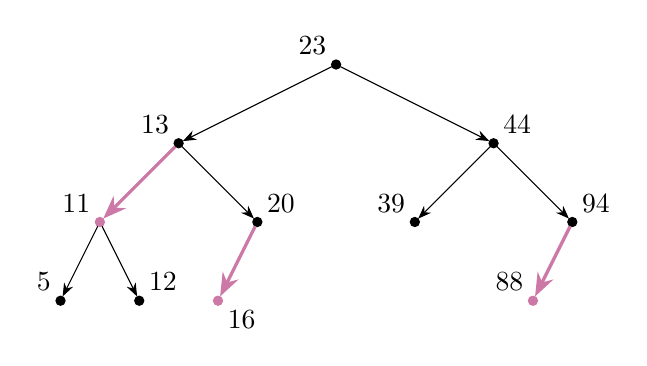
\begin{tikzpicture}
  \node[dot] (p) at (0, 0)       {};
  \node[dot] (l) at (-2, -1)     {}  edge[<-] (p);
  \node[dot,cbReddischPurple] (ll) at (-3, -2)  {}  edge[<-,very thick,cbReddischPurple] (l);
  \node[dot] (lll) at (-3.5, -3) {}  edge[<-] (ll);
  \node[dot] (llr) at (-2.5, -3) {}  edge[<-] (ll);
  \node[dot] (lr) at (-1, -2)  {}  edge[<-] (l);
  \node[dot,cbReddischPurple] (lrl) at (-1.5, -3)  {}  edge[<-,very thick,cbReddischPurple] (lr);
  \node[dot] (r) at (2, -1)     {}  edge[<-] (p);
  \node[dot] (rl) at (1, -2)  {}  edge[<-] (r);
  \node[dot] (rr) at (3, -2) {} edge[<-] (r);
  \node[dot,cbReddischPurple] (rrl) at (2.5, -3) {} edge[<-,very thick,cbReddischPurple] (rr);


  \node[above left] at (p)  {23};
  \node[above left] at (l)  {13};
  \node[above left] at (ll) {11};
  \node[above left] at (lll) {5};
  \node[above right] at (llr) {12};
  \node[below right] at (lrl) {16};
  \node[above right] at (lr) {20};
  \node[above right] at (r)  {44};
  \node[above left] at (rl) {39};
  \node[above right] at (rr) {94};
  \node[above left] at (rrl) {88};
\end{tikzpicture}

\item Draw the red-black tree obtained by adding the values in $S$ in sequence.

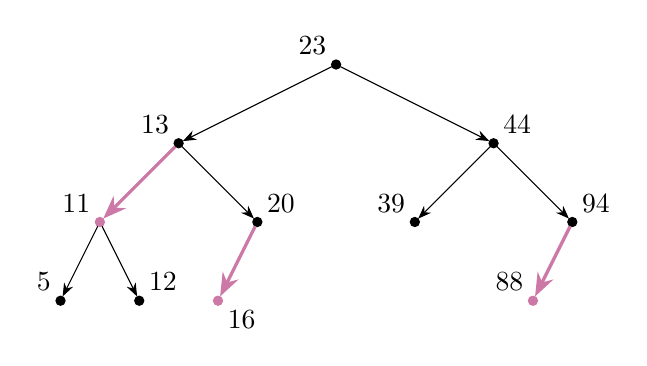
\begin{tikzpicture}
  \node[dot] (p) at (0, 0)       {};
  \node[dot] (l) at (-2, -1)     {}  edge[<-] (p);
  \node[dot,cbReddischPurple] (ll) at (-3, -2)  {}  edge[<-,very thick,cbReddischPurple] (l);
  \node[dot] (lll) at (-3.5, -3) {}  edge[<-] (ll);
  \node[dot] (llr) at (-2.5, -3) {}  edge[<-] (ll);
  \node[dot] (lr) at (-1, -2)  {}  edge[<-] (l);
  \node[dot,cbReddischPurple] (lrl) at (-1.5, -3)  {}  edge[<-,very thick,cbReddischPurple] (lr);
  \node[dot] (r) at (2, -1)     {}  edge[<-] (p);
  \node[dot] (rl) at (1, -2)  {}  edge[<-] (r);
  \node[dot] (rr) at (3, -2) {} edge[<-] (r);
  \node[dot,cbReddischPurple] (rrl) at (2.5, -3) {} edge[<-,very thick,cbReddischPurple] (rr);


  \node[above left] at (p)  {23};
  \node[above left] at (l)  {13};
  \node[above left] at (ll) {11};
  \node[above left] at (lll) {5};
  \node[above right] at (llr) {12};
  \node[below right] at (lrl) {16};
  \node[above right] at (lr) {20};
  \node[above right] at (r)  {44};
  \node[above left] at (rl) {39};
  \node[above right] at (rr) {94};
  \node[above left] at (rrl) {88};
\end{tikzpicture}

\item Consider the hash-function $h(k) = (2k + 5) \bmod 11$ and a hash-table of $11$ table entries that uses hashing with separate chaining. Draw the hash-table obtained by adding the values in $S$ in sequence.


\item Consider the hash-function $h(k) = (3k + 2) \bmod 11$ and a hash-table of $11$ table entries that uses hashing with linear probing. Draw the hash-table obtained by adding the values in $S$ in sequence.


\end{questions}
\end{problem}


\begin{problem}
We say that a hash function $h : \mathcal{U} \rightarrow \mathbb{N}$ that maps values from a set $\mathcal{U}$ to integers in the range $[0\dots M)$ is \emph{$n$-perfect} if there exists at most $n$ distinct values $u_1, \dots, u_j \in \mathcal{U}$ such that $h(u_1) = \dots = h(u_j)$.
\begin{questions}
\item Consider the hash function $h(k) = (2k + 5) \bmod 11$. Is this hash function $2$-perfect for the inputs $0, \dots, 21$? Explain why or why not.

\textbf{Answer:}
This function is 2-perfect for the inputs 0,...,21 since after computation, there is only 2 values mapped to one spot in the hash table. In summary, since the function has 2k, as you loop through the values, the new value will most often be 2 more than the previous. This is until you hit 11 as it is mod 11, then it will start back at either 0 or 1 depending on if the previous value was 9 or 10. The following is the computation.\\

\begin{center}
  \begin{tabular}{||c|c|c|c|c|c|c|c||} 
    \hline
    v & h(v)=(2v+5)mod 11 & v & h(v) & v & h(v) & v & h(v) \\ [0.5ex] 
    \hline\hline
    0 & 5 & 6 & 6 & 12 & 7 & 18 & 8\\ 
    1 & 7 & 7 & 8 & 13 & 9 & 19 & 10 \\
    2 & 9 & 8 & 10 & 14 & 0 & 20 & 1 \\
    3 & 0 & 9 & 1 & 15 & 2 & 21 & 3 \\
    4 & 2 & 10 & 3 & 16 & 4 &  & \\
    5 & 4 & 11 & 5 & 17 & 6 &  & \\ [1ex] 
    \hline
  \end{tabular}
\end{center}

Rearrange to see that there are only two values per mapping. We can see that if there was 1 more value, it would no longer be 2-perfect:

\begin{center}
  \begin{tabular}{||c|c|c|c|c|c|c|c||} 
    \hline
    h(v) & v & h(v) & v & h(v) & v & h(v) & v \\ [0.5ex] 
    \hline\hline
    0 & 3, 14 & 3 & 10, 21 & 6 & 6, 17 & 9 & 13, 2\\ 
    1 & 9, 20 & 4 & 5, 16 & 7 & 12, 1 & 10 & 8, 19 \\
    2 & 4, 15 & 5 & 11, 0 & 8 & 7, 18 &  &  \\ [1ex] 
    \hline
  \end{tabular}
\end{center}


\item Prove that a hash function $h : \mathcal{U} \rightarrow \mathbb{N}$ can only be $n$-perfect if $\abs{\mathcal{U}} \leq n \cdot M$.

\textbf{Answer:}

Assume $h : \mathcal{U} \rightarrow \mathbb{N}$ is n-perfect and let 
$u_1, \dots, u_j$ be j distinct values in $\mathcal{U}$ such that $h(u_1) = \dots = h(u_j)$. Then we will have that $j \leq n$.

$\mathcal{S}_i = \{x \in \mathcal{U}\:|\:h(x) = i\}$ --> In other words, $\mathcal{S}_i$ has elements in $\mathcal{U}$ that map to $i$

This means, $\mathcal{U} = \sum_{i=0}^{M-1} \mathcal{S}_i$ where $|\mathcal{U}| = M$

since $h$ is n-perfect, we know $|\mathcal{S}_i| \leq n$

$\mathcal{U} = \sum_{i=0}^{M-1} \mathcal{S}_i$\\
$|\mathcal{U}| = |\sum_{i=0}^{M-1} \mathcal{S}_i|$\\
$ = \sum_{i=0}^{M-1} |\mathcal{S}_i|$\\
$ \leq \sum_{i=0}^{M-1} n$\\
$ = nM $\\

In conclusion, we have proven that assuming $h : \mathcal{U} \rightarrow \mathbb{N}$ is a n-perfect hash function, then $|\mathcal{U}| \leq nM$ holds.

As we provided an upper bound on the number of elements in $\mathcal{U}$ that can be hashed without collisions, we know that adding any more elements will result in more than n values being mapped to a single hash value, which violates n-perfect rules.

\item Can a general purpose hash function be $n$-perfect for any $M$? Argue why or why not.

\textbf{Answer: }

No a general-purpose hash function cannot be n-perfect for any M because a general-purpose hash function must be able to take in any set of input and ensure each hash value contains $\leq n$ values from the input. 
This means it needs to handle inputs such as lists that have near infinity values (huge M), which is impossible to be n-perfect as you'd have to have an unrealistic number of spots in the hash-table to put the values in.

Mathematically, the Probability a value $V_r$ in the input set collides with a previously hashed value is:

Probability($V_r$ collides with $V_1$) $\cdot$ Probability($V_r$ collides with $V_2$) $\cdot \dots$ Probability($V_r$ collides with $V_{r-1}$)

1/M + 2/M + 3/M... n/M, where n is the $n_{th}$ element in the input list.

FIX THISSSSSSSSSSSSSSSSSSSSSS

the probability to have a collision is $\sim 1 - \frac{n}{M}$

\end{questions}
\end{problem}

\begin{problem}
Consider non-empty binary search trees $T_1$ and $T_2$ such that all values in $T_1$ are smaller than the values in $T_2$. The \AName{SetUnion} operation takes binary search trees $T_1$ and $T_2$ and returns a binary search trees holding all values originally in $T_1$ and $T_2$ (destroying $T_1$ and $T_2$ in the process). 
\begin{questions}
\item Assume the binary search trees storing $T_1$ and $T_2$ have the same height $h$. Show how to implement the \AName{SetUnion} operation in $\OOG{h}$ such that the resulting tree has a height of at-most $h+1$.



\item Assume that $T_1$ and $T_2$ are red-black trees with the same black height $h$. Show how to implement a \AName{SetUnion} operation that returns a red-black tree in $\OOG{h}$.



\item Assume that $T_1$ and $T_2$ are red-black trees with black heights $h_1 > h_2$. Show how to implement a \AName{SetUnion} operation that returns a red-black tree in $\OOG{h_1}$.



\end{questions}
\end{problem}


\begin{problem}
Consider \emph{binary strings} (sequences of zeros and ones). 
\begin{questions}
\item Design a data structure \AName{BSSet} that can be used to represent \emph{sets of binary strings} such that any binary string $W$ of length $\abs{W} = N$ can be added or removed in $\OOG{N}$ and such that one can check whether $W$ is in the data structure in $\OOG{N}$. Sketch why your data structure  \AName{BSSet} supports the stated operations in $\OOG{N}$.
\item Let $W$ of length $\abs{W} = N$ be a binary string and let $S$ be a \AName{BSSet} set. Provide an algorithm that prints all strings $V \in S$ that start with the prefix $W$ (the first $\abs{W}$ characters of $S$ are equivalent to $W$). Your algorithm should have a worst-case complexity of $\OOG{N + k}$ in which $k$ is the number of characters printed to the output.
\item Professor X claims to have developed a data structure \AName{BSSetX} to which any binary string $W$ of length $\abs{W} = N$ can be added in $\OOG{N}$. Furthermore, Professor X claims that \AName{BSSetX}  provides \emph{ordered iteration}: one can iterate over all $M = \abs{S}$ strings in a set $S$, implemented via \AName{BSSetX}, in a lexicographical order in $\OOG{M + T}$ in which $T$ is the combined length of the $M$ strings. Professor X claims that this method of sorting binary strings proves that the worst-case lower bound for sorting $M$ binary strings is \emph{not} $\OOG{M \log_2(M)}$ comparisons. Argue why Professor X is wrong.

We note that strings $S_1$ and $S_2$ are \emph{lexicographical ordered}, denoted by $S_1 \prec S_2$, if $S_1$ comes before $S_2$ in an alphabetical sort (e.g., as used in a dictionary). Next, we formalize $S_1 \prec S_2$ for binary strings: we have $S_1 \prec S_2$ if $S_1$ and $S_2$ are equivalent up to the $0\leq i \leq \min(\abs{S_1}, \abs{S_2})$-th character ($S_1[0] = S_2[0]$,
\dots, $S_1[i-1] = S_2[i-1]$) and either $\abs{S_1} = i < \abs{S_2}$ or the $(i+1)$-th character of $S_1$ comes before the $(i+1)$-th character of $S_2$ (in which case $S_1[i] = 0$ and $S_2[i] = 1$). For example, $0 \prec 00$ and $00 \prec 01$, but not $100 \prec 10$. 
\end{questions}
\end{problem}

\SUBMITMSG{}
\DEFAULTGRADING{}

\end{document}